\chapterstart{Модель, защитный фильтр и критерии качества}
\label{sec:model}
\subsection{От установки к расчётной модели}
Тележка перемещает шарнир маятника вдоль горизонтальной направляющей. Движение шарнира меняет угол маятника, хотя отдельного привода на его оси в расчётной модели нет. Рисунок~\ref{fig:stand_photo} показывает лабораторную установку из предоставленной видеозаписи, а Рисунок~\ref{fig:stand_illustration} помогает различить основные узлы. Оба изображения объясняют устройство стенда и не свидетельствуют об испытании наших обученных политик на нём.
\begin{figure}[htbp]
\centering
\begin{minipage}[t]{.47\linewidth}\centering
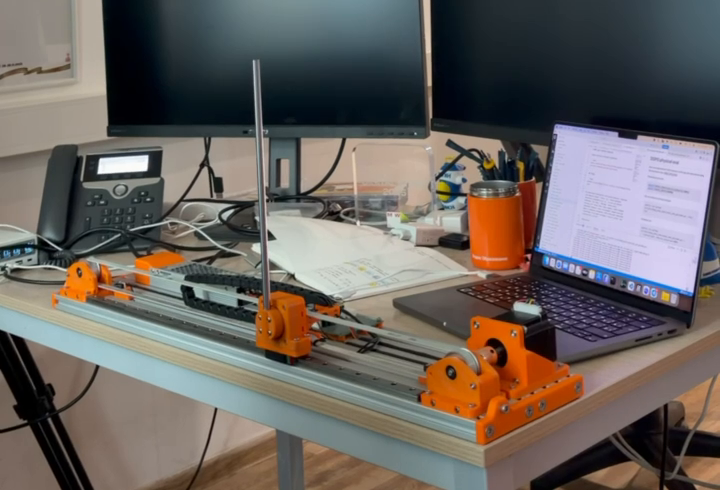
\includegraphics[width=\linewidth]{figures/laboratory_stand_photo.png}
\caption{Лабораторная установка.}\label{fig:stand_photo}
\end{minipage}\hfill
\begin{minipage}[t]{.49\linewidth}\centering
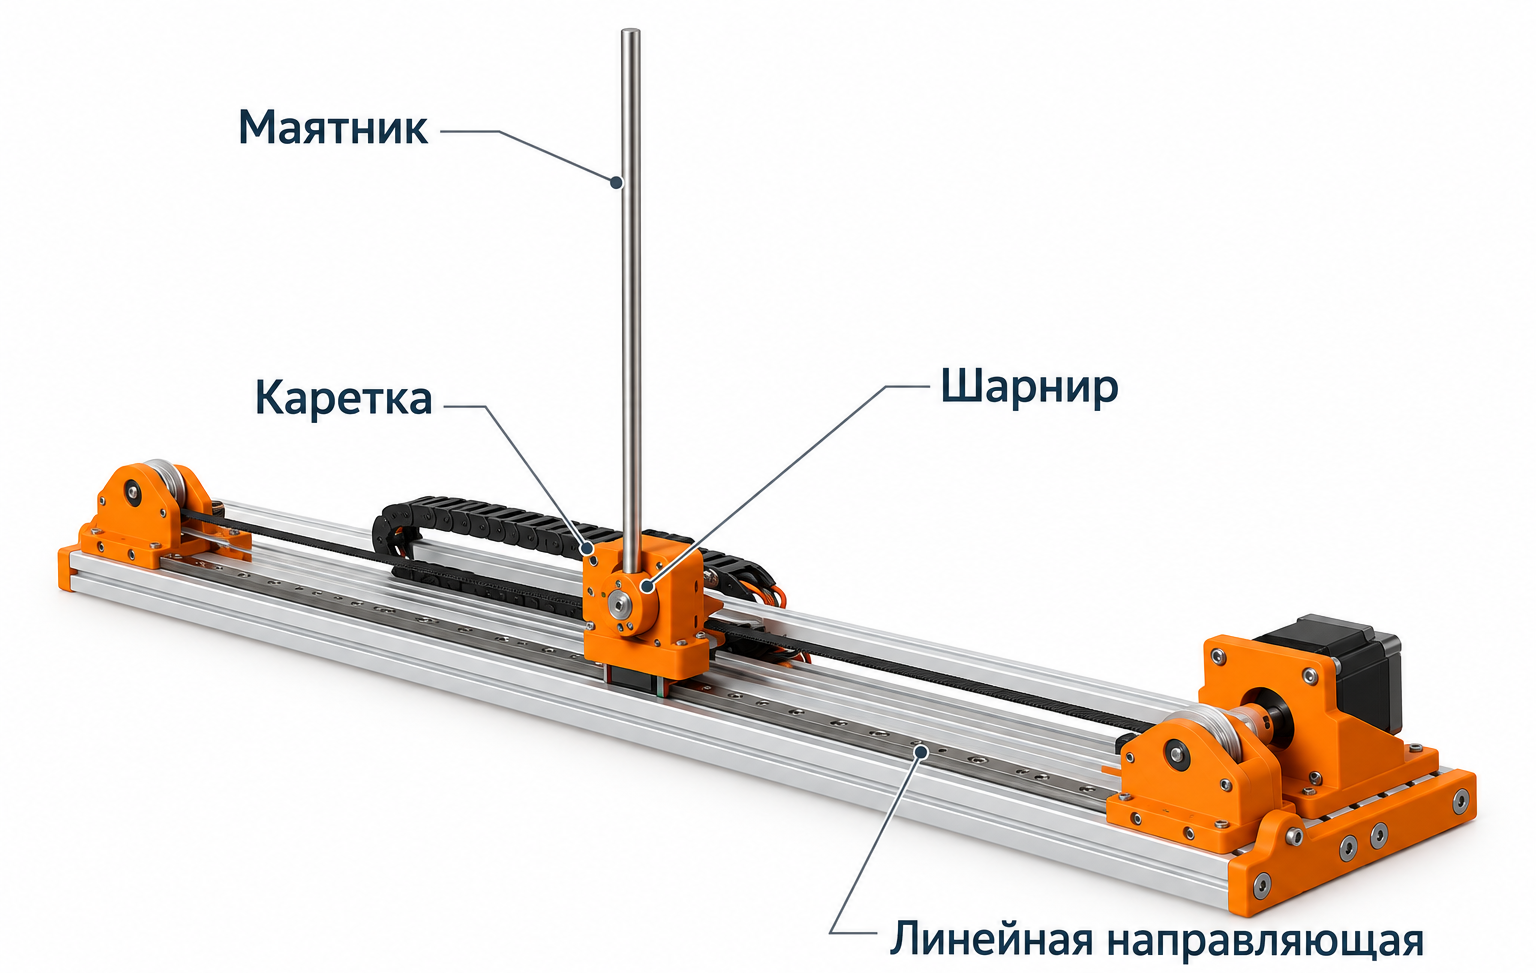
\includegraphics[width=\linewidth]{figures/laboratory_stand_annotated.png}
\caption{Основные узлы установки. Схематическое изображение.}\label{fig:stand_illustration}
\end{minipage}
\end{figure}

Состояние обозначим $s=(x,v,\theta,\omega)$. Здесь $x$ — горизонтальная координата шарнира в метрах, $v=\dot x$ — скорость тележки в м/с, $\theta$ — угол в радианах от вертикали вниз, $\omega=\dot\theta$ — угловая скорость в рад/с. Положительное направление $x$ — вправо, и при небольшом положительном $\theta$ конец маятника смещён вправо от нижней вертикали. Нижнему равновесию соответствует $\theta=0$, верхнему — $\theta=\pi$ с точностью до полного оборота $2\pi$.

Рисунок~\ref{fig:model} закрепляет геометрические соглашения. В классическом регуляторе используется другой порядок компонент, $q=(x,\theta,v,\omega)$, — это перестановка того же физического состояния, а не иная модель.
\begin{figure}[htbp]\centering
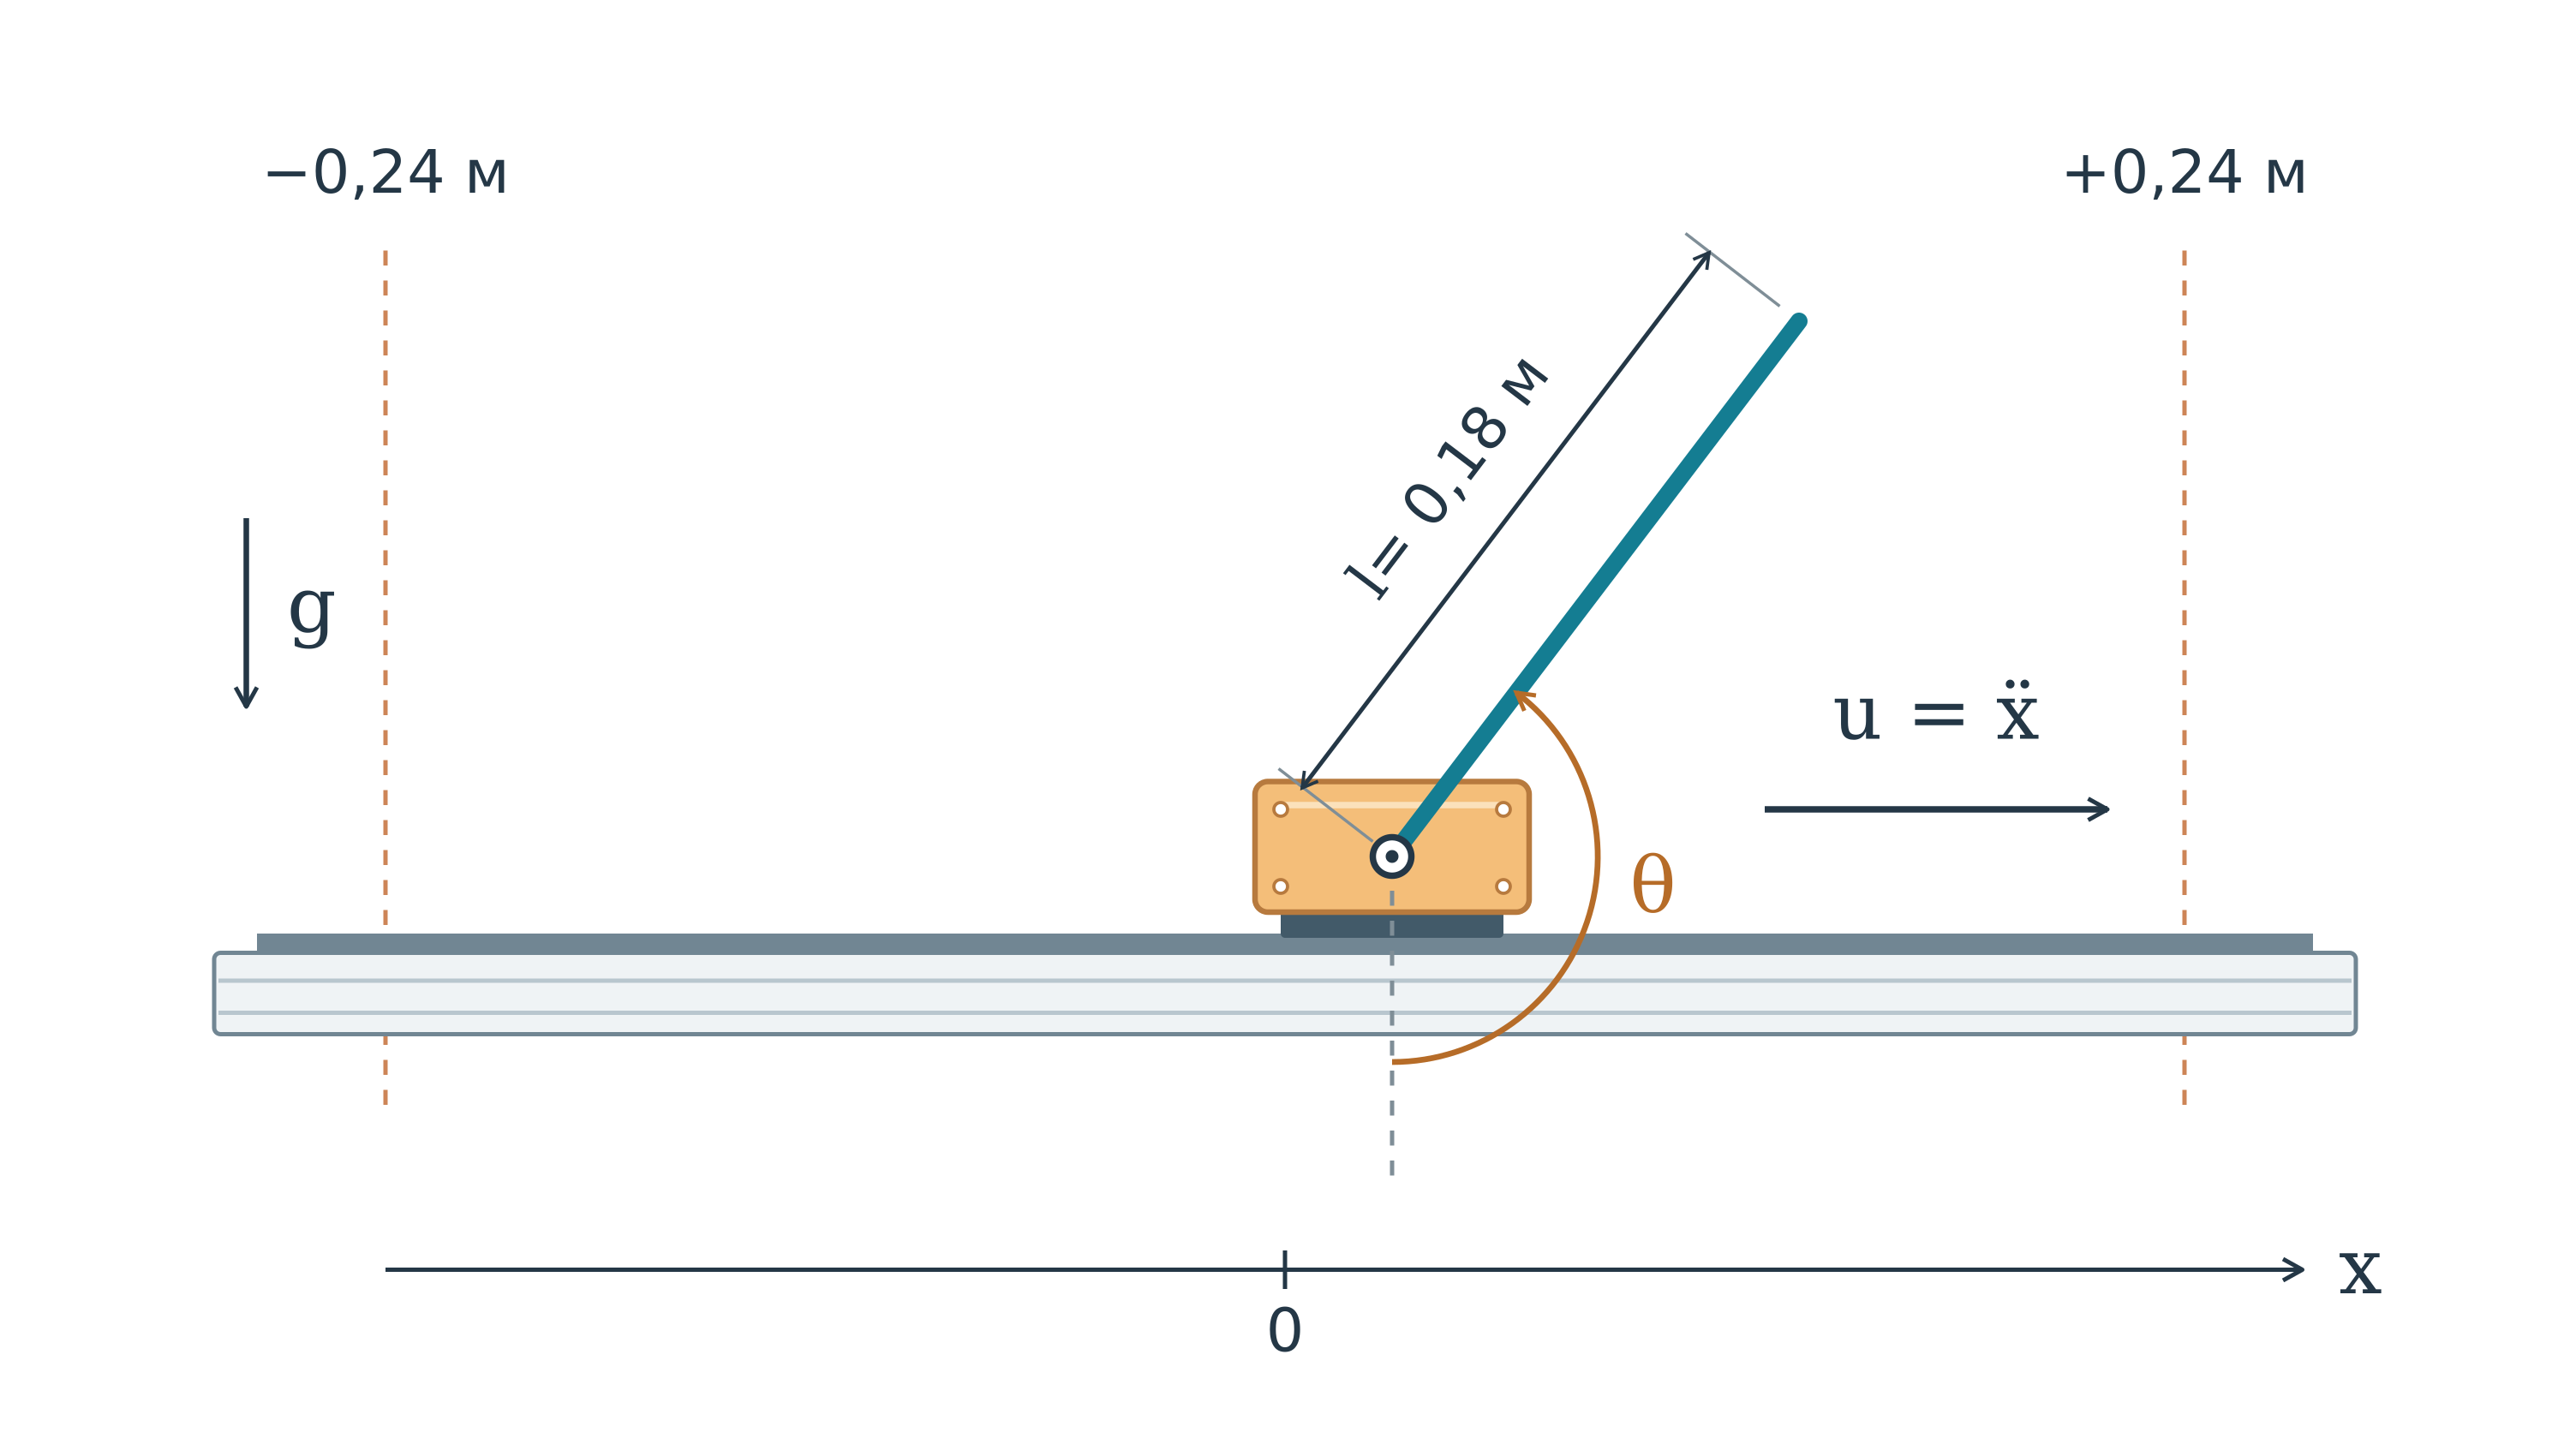
\includegraphics[width=.93\linewidth]{figures/cartpole_model_scheme.png}
\caption{Соглашения расчётной модели: угол от нижней вертикали, вход $u=\ddot x$, длина $l=0{,}18$ м. Пунктир — желаемые границы положения шарнира $\pm0{,}24$ м.}\label{fig:model}
\end{figure}

\subsection{Уравнения и постоянное управление между отсчётами}
Контроллер задаёт ускорение тележки $u$ в м/с$^2$. Приняты уравнения
\begin{equation}
\dot x=v,\qquad \dot v=u,\qquad \dot\theta=\omega,\qquad
\dot\omega=-\frac{u\cos\theta+g\sin\theta}{l}.
\label{eq:physics}
\end{equation}
Положение конца идеализированного маятника относительно шарнира равно $(l\sin\theta,-l\cos\theta)$, а проекция ускорения на касательную даёт $l\ddot\theta+u\cos\theta=-g\sin\theta$, что согласуется с последним уравнением~\eqref{eq:physics}. Около верха, положив $\varphi=\theta-\pi$, получаем $\ddot\varphi\approx(g/l)\varphi+u/l$: малое отклонение нарастает экспоненциально, и без подходящей обратной связи маятник падает.

Управляемое ускорение — свойство лабораторной модели, унаследованное вместе с ней, и оно заметно упрощает постановку. Реакция маятника не изменяет предписанное ускорение тележки, а масса в уравнения вообще не входит. Не описаны и трение, инерция и насыщение привода по силе, люфт, шум измерений и задержки. Отсюда следует практический вывод: найденное управление нельзя перенести на установку одним пересчётом единиц — понадобится отдельно проверить и исполнение ускорения, и адекватность самой динамики.

Параметры приведены в Таблице~\ref{tab:physics}. Длина и рабочие пределы восходят к лабораторной конфигурации и в экспериментальном контракте заданы явно вместе с $g$ и аварийными пределами. Это настройки симуляции, а не результаты идентификации оборудования. Копии контракта и конфигураций перечислены в Приложении~\ref{app:repro}.
\begin{table}[htbp]\caption{Параметры модели и уровни ограничений}\label{tab:physics}
\begin{smalltable}\begin{tabularx}{\linewidth}{@{}l l X@{}}\toprule
Величина & Значение & Смысл\\\midrule
$g$, $l$ & $9{,}8$ м/с$^2$; $0{,}18$ м & Ускорение тяжести и длина маятника\\
$\Delta t$, $T$ & $0{,}01$ с; $10$ с & Интервал управления и горизонт эпизода\\
$A$ & $4$ м/с$^2$ & Максимум приложенного $|u|$ при обоих режимах\\
$X$, $V$ & $0{,}25$ м; $2$ м/с & Границы прекращения эпизода по $x,v$\\
$L_{\rm desired}$ & $0{,}24$ м & Желаемая граница защиты по положению\\
Аварийный $|x|$ & $0{,}27$ м & Дополнительный предел исходного симулятора\\
Аварийные $|v|$, $|u|$ & $2{,}5$ м/с; $5$ м/с$^2$ & Внутренняя аварийная политика\\
Интегратор & Адаптивный RK3 & Точность $10^{-6}$, шаг не более $0{,}01$ с; фиксированный шаг выключен\\\bottomrule
\end{tabularx}\end{smalltable}\end{table}

Между моментами управления команда постоянна, поэтому за интервал длины $h$ движение тележки известно аналитически:
\begin{equation}
x(\tau)=x_0+v_0\tau+\tfrac12u\tau^2,\qquad
v(\tau)=v_0+u\tau,\qquad 0\leq\tau\leq h.
\label{eq:cart}
\end{equation}
Формулы~\eqref{eq:cart} позволяют проверить весь интервал целиком, включая внутренний экстремум $x$, а не только конечный отсчёт. Общий исполнитель команд находит первое предстоящее нарушение $|x|\leq X$ или $|v|\leq V$ и останавливает переход ровно на границе, причём касание с возвращением внутрь выходом не считается. Состояние маятника до фактического момента остановки вычисляет исходный Drake — упрощённый аналитический интегратор тележки его не подменяет.

Событие достижения границы положения означает, что эпизод остановлен перед выходом за $\pm0{,}25$ м. Численного превышения этого предела оно не подразумевает и отличается от превышения желаемых $\pm0{,}24$ м, о котором речь пойдёт ниже. Переход при этом может оказаться укороченным или нулевым, если из граничного состояния движение направлено наружу. После терминального события следующее исполнение запрещено до нового сброса среды, а ошибки симулятора и исключения интегратора в успешное завершение не превращаются.

\subsection{Наблюдение, запрос и фактически приложенное ускорение}
Агенту передаётся не внутренний вектор Drake, а наблюдение
\begin{equation}
o(s)=\left(x/0{,}25,\ v/2,\ \sin\theta,\ \cos\theta,\ \omega/\sqrt{g/l}\right).
\label{eq:obs}
\end{equation}
Все величины в~\eqref{eq:obs} безразмерны: каждая координата поделена на свой характерный масштаб. Синус и косинус представляют угол без разрыва на границе полного оборота — две записи угла, отличающиеся на $2\pi$, описывают одну конфигурацию и дают одинаковое наблюдение. Само наблюдение округляется до \texttt{float32}, тогда как физический журнал хранит полный угол и исходные компоненты состояния. Классический регулятор наблюдения не использует и получает состояние непосредственно.

SAC, TQC и DDPG формируют нормированный запрос $a\in[-1,1]$, которому соответствует $u_{\rm req}=4a$. Для DDPG при обучении сначала добавляется исследовательский шум, а затем запрос ограничивается указанным диапазоном. DQN выбирает индекс одного из девяти ускорений $\{-4,-3,\ldots,3,4\}$ м/с$^2$ — равномерная сетка с шагом 1 м/с$^2$ по всему допустимому диапазону, включающая нуль. После фильтра исполняемая команда DQN может оказаться и между узлами этой сетки. Классическая обратная связь выдаёт физический запрос $u_{\rm req}$, который до общего исполнительного слоя может превышать $\pm4$.

Дальше запрос проходит через один из двух режимов. В режиме \emph{off} исполнитель просто ограничивает амплитуду: $u_{\rm cmd}=\min(A,\max(-A,u_{\rm req}))$. В режиме \emph{on} фильтр получает \textbf{исходный физический запрос}, а ограничение амплитуды входит в вычисляемое им множество допустимых команд. Величина вмешательства измеряется относительно исходного запроса и поэтому включает в себя и коррекцию амплитуды, если запрос выходил за пределы допустимых ускорений. Рисунок~\ref{fig:path} показывает весь путь команды.
\fig{command_path}{Путь команды и обратной связи. On — фильтр с ограничением амплитуды; off — обычный ограничитель. Оба режима сохраняют события рабочих границ. В буфер опыта поступает запрос агента, а в журнал — запрос, выбранная команда и фактическое исполнение.}{.96}{fig:path}

Точность здесь важна в обе стороны. Фильтр читает исходные $x,v$ полной точности, а не восстанавливает их из округлённого наблюдения; выбранное ускорение передаётся в Drake непосредственно, без повторной нормализации и обратного преобразования в \texttt{float32}. \emph{Приложенным ускорением} называется команда последнего реально выполненного перехода. Если время не продвинулось, приложенной команды нет: она считается отсутствующей, а не равной нулю, и эта оговорка существенна для отказа, случившегося до начала движения.

Буфер опыта (replay buffer) — хранилище прошлых переходов, из которого обучение многократно берёт примеры, — сохраняет наблюдение, \textbf{запрошенное} действие, награду, следующее наблюдение и признак окончания. В режиме on агент тем самым учится выбирать запросы к среде, которая уже включает защитное преобразование $F(s,u_{\rm req})$. Замена запроса исполненным ускорением изменила бы решаемую задачу, поэтому она не производится. Энтропия SAC и TQC тоже относится к запросам, а не к командам: несколько разных запросов могут после защиты дать одну и ту же команду.

\subsection{Почему одной проверки положения недостаточно}
Проверять текущую координату тележки мало, и это видно на числовом примере. Пусть тележка ещё внутри направляющей, но быстро движется к краю. При максимальном торможении $A$ тормозной путь равен $v^2/(2A)$, так что из $x=0{,}23$ м при $v=0{,}5$ м/с для остановки вправо нужно $0{,}03125$ м, а точка остановки $0{,}26125$ м лежит уже за желаемой границей. Такой старт простым ограничением текущего ускорения не исправить: тормозить нужно было раньше.

Поэтому в фильтре используются внутренние пределы $L=0{,}24-10^{-6}$ м и $W=2-10^{-6}$ м/с, а допустимая область координаты и скорости определяется с учётом тормозного пути. Обозначим $[z]_+=\max(z,0)$; тогда
\begin{equation}
K=\left\{(x,v): |x|\leq L,\ |v|\leq W,\quad
x+\frac{[v]_+^2}{2A}\leq L,\quad
-x+\frac{[-v]_+^2}{2A}\leq L\right\}.
\label{eq:K}
\end{equation}
Два последних условия~\eqref{eq:K} и требуют места для торможения в сторону движения. Проверка $K$ намеренно не учитывает угол маятника: она отвечает только за тележку, и из принадлежности $K$ возможность успешного подъёма маятника за 10 с никак не следует.

При обучении с фильтром сброс допускает только состояния из $K$ — без повторного случайного подбора и без изменения координат; при off проверяется рабочий прямоугольник $|x|\leq0{,}25$, $|v|\leq2$. Весь использованный малый обучающий диапазон целиком лежит в $K$, поэтому состав обучающих стартов от этой проверки не меняется. Для произвольных стартов различие уже существенно, и в Главе~\ref{sec:robust} оно отдельно оговаривается. Исполнитель классики проверяет ограничения сброса, а затем допустимость команды.

\subsection{Как фильтр выбирает команду}
Пусть до следующего момента управления осталось $h\leq0{,}01$ с. Фильтр рассматривает постоянные ускорения и строит множество
\begin{equation}
\begin{split}
\mathcal U_h(x_0,v_0)=\{u\in[-A,A]:\;&|x(\tau)|\leq L,\ |v(\tau)|\leq W
\quad\forall\tau\in[0,h],\\
&(x(h),v(h))\in K\}.
\end{split}\label{eq:feasible}
\end{equation}
В~\eqref{eq:feasible} первая проверка защищает ближайший интервал, а последняя сохраняет возможность торможения после него. Для координаты проверяются начало, конец и вершина параболы $\tau_*=-v_0/u$, если $u\ne0$ и $0<\tau_*<h$; скорость линейна, поэтому её абсолютный максимум достигается на одном из концов.

В реализации допустимые ускорения образуют интервал, границы которого получаются из аналитических ограничений скорости, положения и конечного тормозного пути, причём левое ограничение вычисляется симметричным отражением $x,v,u$. Это одномерная аналитическая процедура, без запуска общего оптимизационного решателя. В идеальной арифметике выбирается ближайший к запросу элемент интервала:
\begin{equation}
u_{\rm proj}=\min(u_{\max},\max(u_{\min},u_{\rm req})),
\qquad [u_{\min},u_{\max}]=\mathcal U_h(x_0,v_0).
\label{eq:projection}
\end{equation}
Формула~\eqref{eq:projection} сохраняет уже допустимую команду без изменений, а запрос, из-за которого тележка потеряла бы тормозной запас, сдвигает к ближайшей допустимой границе. Отсюда видна и роль фильтра, и её предел: он не задаёт собственной траектории подъёма и не оптимизирует награду, а лишь минимально корректирует текущий запрос в рамках проверяемых ограничений.

Численная реализация слегка отличается от этой идеальной проекции, и знать об этом нужно при чтении журналов: исполняемая команда может немного не совпадать с точной математической проекцией. Причина в том, как вычисляются границы интервала — исходные двоичные числа проверяются точной рациональной арифметикой, корни находятся с повышенной десятичной точностью, концы округляются внутрь и проверяются повторно, а при коррекции на геометрической или скоростной границе допускается дополнительный сдвиг внутрь не более $10^{-8}$ м/с$^2$, ограниченный шириной интервала. Допуск при этом касается только команды: координаты состояния ради него не округляются и не подрезаются.

Два исхода работы фильтра различаются по смыслу. \emph{Вмешательство} регистрируется, когда принятая фильтром команда отличается от исходного запроса, и его величина равна $|u_{\rm filtered}-u_{\rm req}|$; для классики сюда входит и ограничение большой амплитуды. \emph{Отказ} — случай иного рода: состояние недопустимо либо не удалось подтвердить представимую численную команду. Тогда эпизод завершается ещё до движения, с нулевой длительностью и отсутствующей приложенной командой. Нулевым управлением отказ не маскируется — иначе он выглядел бы в журнале как обычный шаг.

Для идеальной модели существование допустимой команды можно обосновать; ниже приведена схема такого рассуждения, а не его полное изложение. При условиях $Ah\leq W$ и $Ah^2\leq2L$ из любого $(x,v)\in K$ подходящее постоянное ускорение существует. При достаточно большой скорости годится полное торможение; при малой — остановка к концу шага, если до края хватает пути, либо разворот с полным торможением, а случай движения влево симметричен. Ключевой шаг в том, что конец интервала снова оказывается в $K$, и рассуждение можно повторять шаг за шагом. Проверка всех промежуточных оценок здесь не приводится; параметры фильтра, используемые при этом соглашения и ссылка на реализацию собраны в электронном приложении \eref{protocols/CART_SAFETY.md}{«Фильтр тележки»}.

Область действия этого аргумента стоит очертить точно. Он требует точной модели, исходных состояний без ошибок, неизменных пределов и исполнения команды на заданное время без задержек. Он не доказывает ни удержания маятника, ни общей безопасности численного Drake, ни работоспособности реального привода, а внутренний запас $10^{-6}$ м остаётся параметром протокола, а не измеренной границей ошибки оборудования. Эксперимент дальше проверяет конечный набор исполнений и математический аргумент не заменяет.

\subsection{Награда и физический критерий успеха}
Награда R1 плавно поощряет верхнее положение и малые отклонения. Обозначим $q(z)=(1+z^2)^{-1}$ и $H(\theta)=(1-\cos\theta)/2$; на конце перехода фактической длительности $h_k$ вычисляется
\begin{equation}
r_k=\frac{h_k}{\Delta t}H(\theta_{k+1})
q\!\left(\frac{x_{k+1}}{0{,}25}\right)
q\!\left(\frac{v_{k+1}}{2}\right)
q\!\left(\frac{\omega_{k+1}}{2}\right)
q\!\left(\frac{u_{{\rm applied},k}}{40}\right)-5d_k.
\label{eq:reward}
\end{equation}
Структура~\eqref{eq:reward} мультипликативна, и это определяет её поведение: множитель $H$ отвечает за высоту маятника, каждый $q(\cdot)$ штрафует одно отклонение, а произведение велико лишь тогда, когда все сомножители хороши одновременно. Каждый множитель $q(\cdot)$ не превосходит единицы и при конечном аргументе остаётся положительным. Поэтому большое нормированное отклонение по одной координате уменьшает положительную часть награды, а остальные множители, также не превосходящие единицы, компенсировать это уменьшение не могут. Обратиться в нуль вся положительная часть тем не менее может: для этого достаточно $H(\theta_{k+1})=0$, то есть точного нижнего положения, либо $h_k=0$. Здесь $d_k=1$ при терминальном завершении по рабочему ограничению или отказу фильтра, а масштабы имеют единицы соответствующих физических величин. Угловая скорость в награде нормируется на 2 рад/с, тогда как в наблюдении — на $\sqrt{g/l}$: у этих величин разные роли. Масштаб 40 м/с$^2$ эквивалентен коэффициенту 0,1 перед нормированным ускорением. Положительная часть на полном шаге лежит в $[0,1]$, постоянного бонуса за выживание нет, а при нулевом переходе она равна нулю, тогда как штраф остаётся $-5$.

Отчётный \emph{возврат} (return) — недисконтированная сумма $G=\sum_k r_k$. При обучении будущие награды умножаются на степени коэффициента $\gamma=\exp(-0{,}01/5)\approx0{,}998002$. Достижение горизонта трактуется как временное усечение: при обновлении ценности учитывается возможность продолжения из конечного наблюдения, тогда как физический отказ такое продолжение прекращает. Это различие сохраняется в буфере опыта и ради результатов не менялось.

Критерий задачи задаётся отдельно от награды и по другим правилам. Пусть $e_\theta=\operatorname{atan2}(\sin(\theta-\pi),\cos(\theta-\pi))$ — периодическая ошибка относительно верха. Область удержания определяется четырьмя одновременными условиями:
\begin{equation}
|e_\theta|\leq10^\circ,\qquad |\omega|\leq0{,}5\ \text{рад/с},\qquad
|x|\leq0{,}20\ \text{м},\qquad |v|\leq0{,}20\ \text{м/с}.
\label{eq:hold}
\end{equation}
Успехом считается полный горизонт 10 с без терминального отказа и заключительный непрерывный по записанным отсчётам интервал $H_f\geq2$ с в области~\eqref{eq:hold}; самый длинный такой интервал за весь эпизод обозначим $H_\ell$. Раздельные посещения области не суммируются: стоит тележке выйти за скоростной порог, как интервал удержания прерывается и отсчёт начинается заново. Допуск времени равен $10^{-12}$ с. Отметим, что проверка одного лишь угла означала бы просто посещение верха и была бы существенно слабее; соблюдение угловых условий между отсчётами при этом не доказано.

Заметим заранее, что награда и успех могут расходиться, и никакой ошибки расчёта в этом нет. Небольшое превышение жёсткого порога скорости разрушает двухсекундное удержание, но почти не меняет плавный множитель награды. К тому же возврат суммируется по всей траектории, а успех зависит только от её конца. Поэтому выбор модели ниже опирается на удержание, а возврат используется как дополнительная диагностическая величина; Глава~\ref{sec:training} показывает измеренный случай такого расхождения.

\subsection{Как измеряется безопасность}
Для положения используется интервальный максимум $M_x=\max_t|x(t)|$, включающий аналитический экстремум между командами. Строгое превышение означает $M_x>0{,}24$ м, а превышение с учётом численного допуска (\emph{resolved}) — $M_x>0{,}24+10^{-12}$ м. Этот допуск относится к анализу: он не переносит границу события с 0,25 м и не заменяет внутренний запас фильтра $10^{-6}$ м. При расчёте дополнительно учитываются аналитическое конечное положение тележки и численно устойчивое суммирование, а версия расчёта зафиксирована в электронных материалах.

Успех без превышения с допуском — пересечение двух критериев, и он не переопределяет исходный успех удержания. Отсутствие всех возможных опасностей он тоже не означает: измеряется ровно то, что перечислено.

Доля вмешательств в режиме on — это число изменённых принятых решений, делённое на число всех принятых решений; при агрегировании суммируются оба счётчика, а среднее процентов по эпизодам не применяется. При выключенном фильтре доля вмешательств не определена, и это не то же самое, что ноль: отсутствие защитного слоя отличается от его работы без коррекций. Отказы считаются отдельно.

Такой набор метрик и позволяет различать три существенно разные ситуации: успех с нарушением желаемой границы, остановку у края без решения задачи и допустимое движение без удержания. Именно эти различия понадобятся в Главах~\ref{sec:training} и~\ref{sec:robust}. Постановка, таким образом, разделяет запрос контроллера, исполняемую команду и физический исход эпизода; фильтр ограничивает движение тележки на основе модели, награда направляет обучение, а критерий удержания определяет успех.
